\section{Bytestrings}
\label{bytestrings}

The Coq \ty{string} type
is defined as a linked list of \ty{ascii}, each of which is record of 8 \ty{bool}s:
\begin{Verbatim}
\kw{Inductive} \ty{ascii} := 
| \dt{Ascii} : \ty{bool} -> \ty{bool} -> \ty{bool} -> \ty{bool} -> \ty{bool} -> \ty{bool} -> \ty{bool} -> \ty{bool} -> \ty{ascii}.
\end{Verbatim}

\begin{Verbatim}
\kw{Inductive} \ty{string} := 
| \dt{EmptyString} : \ty{string} 
| \dt{String} : \ty{ascii} -> \ty{string} -> \ty{string}.
\end{Verbatim}

As we have seen in \autoref{memoryrepresentation}, each \dt{String} constructor is represented as
three words (a header and two pointers), and
each \dt{Ascii} constructor is nine words,
in which each \ty{bool} is \gls{unboxed}. This means when a value of the Coq type \ty{string} is compiled to C, our system uses 96 bytes (on a 64-bit system) per ASCII character, which clearly is inefficient.
Instead, we can introduce a \gls{foreign type} for bytestrings, where each character would occupy one byte (as they do in OCaml~\cite[Chapter 23, ``string values'']{madhavapeddy2022real}), and provide \gls{foreign function}s to convert between this \gls{foreign type} and the Coq \ty{string}s, and operations on this \gls{foreign type}.

In this section, we implement such a \gls{foreign type} and its \gls{foreign function}s. The VST proofs for these functions are written by Stark and Appel, and are covered in the tech report by Korkut, Stark, and Appel~\cite{korkutStarkAppel}.

\subsection{The Coq Interface}

We start by defining a \kw{Module Type}, \ty{Bytestring}, that contains the \gls{foreign type}s and \gls{foreign function}s we need to implement bytestrings.

\begin{Verbatim}
\kw{Module Type} \ty{Bytestring}.
  \kw{Parameter} \ty{bytestring} : \ty{Type}.
  \kw{Parameter} \fn{pack} : \ty{string} -> \ty{bytestring}.
  \kw{Parameter} \fn{unpack} : \ty{bytestring} -> \ty{string}.
  \kw{Parameter} \fn{append} : \ty{bytestring} -> \ty{bytestring} -> \ty{bytestring}.
\kw{End} \ty{Bytestring}.
\end{Verbatim}

We proceed by defining a module, \ty{C} that satisfies the \ty{Bytestring} interface. This module states that all values in the \ty{Bytestring} interface will be \gls{foreign type}s and \gls{foreign function}s.

\newpage
\begin{Verbatim}
\kw{Module} \ty{C} : \ty{Bytestring}.
  \kw{Axiom} \ty{bytestring} : \ty{Type}.
  \kw{Axiom} \fn{pack} : \ty{string} -> \ty{bytestring}.
  \kw{Axiom} \fn{unpack} : \ty{bytestring} -> \ty{string}.
  \kw{Axiom} \fn{append} : \ty{bytestring} -> \ty{bytestring} -> \ty{bytestring}.
\kw{End} \ty{C}.
\end{Verbatim}

We have to register with CertiCoq the \gls{foreign function}s and the names of C functions that will realize those \gls{foreign function}s when a client program is compiled to C.

\begin{Verbatim}
\kw{CertiCoq Register}
  [ \fn{C.pack} => \dt{"pack"} \kw{with tinfo},
  , \fn{C.unpack} => \dt{"unpack"} \kw{with tinfo},
  , \fn{C.append} => \dt{"append"} \kw{with tinfo},
  ] \kw{Include} [ \dt{"prims.h"} ].
\end{Verbatim}

\subsection{The C Implementation}

For brevity, let us explain only the C implementation of the \fn{C.pack} function out of these \gls{foreign function}s. This function converts a Coq \ty{string} into our \gls{foreign type} \ty{C.bytestring}. To understand how this function would be implemented in C, we have to grasp the memory representations of these types.

We have already discussed the memory representation of the \ty{string} type, as it is just another \gls{inductive type}. 
Once we add \ty{string} to the list of types to generate \gls{glue code} about, we will have the \ty{string} counterparts of all the helper functions we went over in \autoref{glue}.

The memory representation of \ty{C.bytestring} will be more complicated. For further compatibility with the OCaml ecosystem, we use the same bytestring representation as OCaml.
We would have the following memory representation (in a 64-bit setting) for the bytestring \dt{\textquotedbl{}interface\textquotedbl{}}:

\begin{figure}[H]
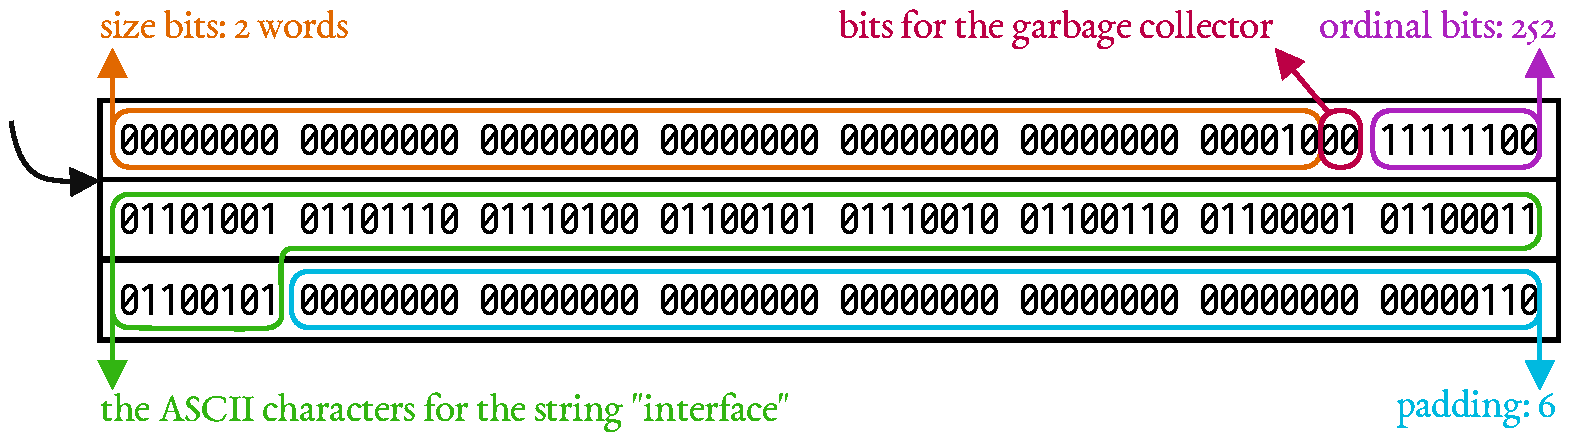
\includegraphics[scale=.55]{figures/bytestring.pdf}
\centering
\caption{The representation of the bytestring \dt{\textquotedbl{}interface\textquotedbl{}} in memory.}
\end{figure}


This string's representation consists of 3 words, one for the header and the remaining two for the characters and padding. After the header, we use one byte per ASCII character, terminated by a null byte. However, our runtime system assumes that values consist of words in memory, and our number of character bytes might not line up with the word size. We alleviate this discrepancy by filling the remaining bytes in the word with a padding. This padding consists of null bytes, with the last byte containing how many extra null bytes had to be added. If the characters and the terminating null byte perfectly fit in words, the last byte is a null byte, which serves both as the terminating byte and also the number of extra null bytes that had to be added.

The header contains the size of the string content, which is 2 words in this example. The last part of the header contains the number $252$, which is a special tag for bytestrings in OCaml. This tag indicates that none of the words in the record are pointers---none should be traversed by the garbage collector---so they don't need to use the last bit of each word to distinguish pointers from integers.

Finally, just as it is the case for all other values in our memory representation, the header is one word behind where the pointer points to.

Now that we understand how bytestrings are supposed to be represented in memory, we can start the C implementation.
We can start with defining an \kw{enum} for the possible \constructor{}s of the Coq type \ty{string}:

\begin{Verbatim}
\kw{typedef} \kw{enum} \{ \dt{EMPTYSTRING}, \dt{STRING} \} \ty{string};
\end{Verbatim}

Here is what the implementation for \fn{C.pack} looks like:

\begin{Verbatim}
\ty{value} \fn{pack}(\kw{struct} \ty{thread_info *}\tinfo{}, \ty{value} \bn{save0}) \{
  \kw{BEGINFRAME}(\tinfo{}, \dt{1})

  \cm{// Allocate enough memory}
  \ty{value} \bn{temp} = \bn{save0};
  \ty{size_t} \bn{i}, \bn{len} = \dt{0};
  \kw{while} (\fn{get_Coq_Strings_String_string_tag}(\bn{temp}) \fn{=}\fn{=} \dt{STRING}) \{
    \bn{len}\fn{+}\fn{+};
    \bn{temp} = \fn{get_args}(\bn{temp})[\dt{1}];
  \} 
  \ty{size_t} \bn{mod} = \bn{len} \fn \kw{sizeof}(\ty{value}));
  \ty{size_t} \bn{nalloc} = (\bn{len} \fn{+} \bn{pad_length}) \fn{/} \kw{sizeof}(\ty{value}) \fn{+} \dt{1ULL};
  \kw{GC_SAVE1}(\bn{nalloc})

  \ty{value *}\bn{argv} = \tinfo{}->\bn{alloc};
  \bn{argv}[\dt{0LLU}] = (\ty{value})(((\bn{nalloc} \fn{-} \dt{1}) \fn{<<} \dt{10}) \fn{+} \dt{252LLU}); \cm{// string tag}

  \cm{// Make the characters}
  \ty{char *}\bn{ptr} = (\ty{char *}) (\bn{argv} \fn{+} \dt{1LLU});
  \bn{temp} = \bn{save0};
  \kw{while} (\fn{get_Coq_Strings_String_string_tag}(\bn{temp}) \fn{==} \dt{1}) \{
    *\bn{ptr} = \fn{ascii_to_char}(\fn{get_args}(\bn{temp})[\dt{0}]);
    \bn{ptr}\fn{+}\fn{+};
    \bn{temp} = \fn{get_args}(\bn{temp})[\dt{1}];
  \}
\end{Verbatim}
\newpage
\begin{Verbatim}
  \cm{// Make the padding}
  \kw{for} (\bn{i} = \dt{0}; \bn{i} \fn{<} \fn{pad_length} \fn{-} \dt{1}; \bn{i}\fn{+}\fn{+}) \{
    \bn{ptr}[\bn{i}] = \dt{0};
  \}
  \bn{ptr}[\bn{i}] = \bn{i};

  \tinfo{}->\bn{alloc} += \bn{nalloc};
  \kw{return} (\ty{value}) (\bn{argv} \fn{+} \dt{1LLU});
  \kw{ENDFRAME}
\}
\end{Verbatim}

This function performs the following steps:
\begin{enumerate}
\item traverses the Coq \ty{string} once to compute its length, stored in \bn{len}
\item makes sure there are $n=1+\lceil (\bn{len}+1)/8\rceil$ words in the \gls{CertiCoq heap}, where it can place the bytestring
\item makes the bytestring header using the special tag and the number of words needed for the bytestring content
\item makes the character by traversing the Coq \ty{string} and converting each C \ty{char} to a Coq \ty{ascii}, by calling the \fn{ascii\_to\_char} function, which we have implemented by hand but omit here
\item makes the padding by adding null bytes, followed by how many extra null bytes had to be added
\item returns a pointer to the first character byte.
\end{enumerate}

Our implementations of \fn{C.unpack} and \fn{C.append} are similar to the implementation of \fn{C.pack} that we presented here. To summarize, \fn{C.unpack} traverses all the character bytes in the bytestring and creates \ty{ascii} and \ty{string} values, using the \gls{glue code}. \fn{C.append} computes the lengths of both of its inputs, allocates enough words in the \gls{CertiCoq heap}, copies characters, and adds padding.

\subsection{The Functional Model}

The simplest way to model bytestrings in Coq is to define them as Coq \ty{string}s. This makes the \gls{functional model}s of all the functions that operate of our \gls{foreign type} trivial:

\begin{Verbatim}
\kw{Module} \ty{FM}.
  \kw{Definition} \ty{bytestring} : \ty{Type} := \ty{string}.
  \kw{Definition} \fn{pack} (\bn{x} : \ty{string}) : \ty{bytestring} := \bn{x}.
  \kw{Definition} \fn{unpack} (\bn{x} : \ty{bytestring}) : \ty{string} := \bn{x}.
  \kw{Definition} \fn{append} (\bn{x} \bn{y} : \ty{bytestring}) : \ty{bytestring} := \fn{append} \bn{x} \bn{y}.
\kw{End} \ty{FM}.
\end{Verbatim}

A curious reader might wonder why we did not address the length of the bytestring in our \gls{functional model}. This would be a fair question, given that we \emph{have} addressed a similar restriction in the \gls{functional model} for integers, in \autoref{integers}. Our answer in this case is practicality. In the memory representation above, we showed that the bytestring header contains 54 bits (in a 64-bit setting) for the size of the string, in words. Thus, the largest bytestring we can create will have $(2^{54})\cdot{}8$, or $2^{57}$ bytes, which is $128$ petabytes.
For \fn{C.pack}, we would need to start with a Coq \ty{string}. In order to reach a bytestring that is $128$ petabytes, at $2$ words per record, we would need $2\cdot{}8\cdot{}2^{57} = 2^{61}$ bytes of memory, i.e.\ $\approx{}2.3$ exabytes.\footnote{This question and its answer was observed by Appel.}  Here we are assuming we are not going to run Coq functions on memories that large, but it is also possible to design a \gls{functional model} for bytestrings in a way that would account for the maximum length.\footnote{In such a design, the \fn{pack} function would have decide how to treat the inputs that would create bytestrings larger than what the bytestring representation could handle. The \fn{pack} function could choose to return only the part that fits in memory, or it could choose to return an \ty{option} value, etc.}

We will not present any proofs about the models for the \gls{foreign function}s on \ty{bytestring}s since our model is trivial and all proofs will simply be about Coq \ty{string}s.